\documentclass[a4paper,twoside,11pt]{article}
\usepackage{graphicx,fancyhdr,amsmath,amssymb,float, caption, hyperref}

%----------------------- Macros and Definitions --------------------------

\setlength\headheight{20pt}
\addtolength\topmargin{-10pt}
\addtolength\footskip{20pt}

\newcommand{\R}{{\mathbb R}}
\newcommand{\dir}{\vec{d}}
\newcommand{\pol}{{\cal P}}
\newcommand{\robot}{{\cal R}}
\newcommand{\triang}{{\cal T}}
\newcommand{\dist}{\mathrm{dist}}
\newcommand{\eps}{\varepsilon}
\newcommand{\Mid}{:}
\newcommand{\ch}{\mathcal{CH}}
\newcommand{\exercise}[1]{\noindent{\bf Exercise #1:}}
\newenvironment{solution}{\begingroup\Solenv}{\END\endgroup}
\def\Solenv{\vspace{.5\baselineskip}\penalty100\advance\leftskip by\parindent
  \advance\leftmargini by\parindent
  \Sol\ \ignorespaces}
\def\Sol{\noindent{\bf Solution\/:}\nobreak}
\def\END{\unskip~\medbreak\medbreak\medbreak}
\def\qed{\hfill$\Box$}

\newtheorem{theorem}{Theorem}
\newtheorem{lemma}[theorem]{Lemma}

\fancypagestyle{plain}{%
\fancyhf{}
\fancyhead[LO,RE]{\sffamily Eindhoven University of Technology}
\fancyhead[RO,LE]{\sffamily }
\fancyfoot[LO,RE]{\sffamily Department of Mathematics \& Computer Science}
\fancyfoot[RO,LE]{\sffamily\bfseries\thepage}
\renewcommand{\headrulewidth}{0pt}
\renewcommand{\footrulewidth}{0pt}
}

\pagestyle{fancy}
\fancyhf{}
\fancyhead[RO,LE]{\sffamily }
\fancyhead[LO,RE]{\sffamily Eindhoven University of Technology}
\fancyfoot[LO,RE]{\sffamily Department of Mathematics \& Computer Science}
\fancyfoot[RO,LE]{\sffamily\bfseries\thepage}
\renewcommand{\headrulewidth}{1pt}
\renewcommand{\footrulewidth}{0pt}

%redefinition of matrix so you can use for example \begin{pmatrix}[rowHeight]
\makeatletter
\renewcommand*\env@matrix[1][\arraystretch]{%
  \edef\arraystretch{#1}%
  \hskip -\arraycolsep
  \let\@ifnextchar\new@ifnextchar
  \array{*\c@MaxMatrixCols c}}
\makeatother

%-------------------------------- Title ----------------------------------

\title{\rule{\linewidth}{.75pt} \center{Title goes here}}
\author{Stefan Patelski}
% \date{}

%--------------------------------- Text ----------------------------------

\begin{document}
\maketitle
\vspace{-2\baselineskip}

\bigskip
\noindent\rule[2.5pt]{\textwidth}{0.75pt}

\newpage

\section{Introduction}

\subsection{Crawler : S.R. Patra}
\subsubsection{Motivation}
The very first task was to collect data for our project. We decided to implement a focused crawler for Rotten tomatoes website to collect information about different movies. Large collection of movies with credible reviews made Rotten Tomatoes a suitable candidate for us to get our data from. The goal was to start with a seed URL and extract all the yet unseen URLs on that HTML page along with the metadata about the movie such as movie name, director, producers,reviews etc. The process needs to be repeated for all the collected links.
\subsubsection{Approach}
For each page, the method \textit{CollectData} in the crawler read the HTML content line by line, only collecting the relevant information and disregarding all the other content that were not relevant to us. This was done with the help of an HTML parser which used \textit{Jsoup} library functions. Whenever relevant data were encountered, they were appended to an XML document. To find the movie URLs , Java's pattern matching functionality was being used which looks for a particular pattern of anchor texts which are specific to movie pages. The crawler architecture is shown in fig.\ref{fig:architecture}.

\begin{figure}[H]
    \centering
    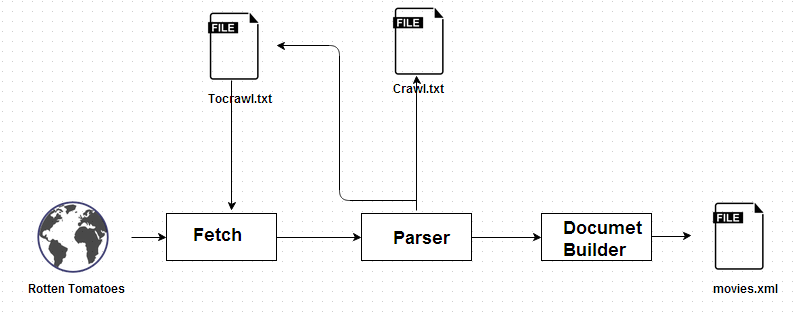
\includegraphics[width=4.0in]{crawler_arch.png}
    \caption{Crawler Architecture}
    \label{fig:architecture}
\end{figure}

\subsubsection{Challenges}
The main challenge was to encounter the non uniformity of the content in Rotten Tomatoes web pages. Some of the web pages contained all the information about the movies while in others, a few of the information fields were missing. The crawler was designed to scrap the HTML data in a way such that maximum amount of information can be retrieved. Another challenge was to make sure that the crawler is not blocked by the site. This was handled by building the crawler in a flexible way so that, during an iteration, the crawler will only crawl through a specific number of pages specified to it as a parameter. After each iteration, the URLs which are already crawlled and the URLs those are yet to be crawlled are written back to \textit{Crawl.txt} and \textit{Tocrawl.txt} respectively which will be used in the next iterations. Fig.\ref{fig:xmlFile} shows an entry in the \textit{movies.xml} file.

\begin{figure}[H]
    \centering
    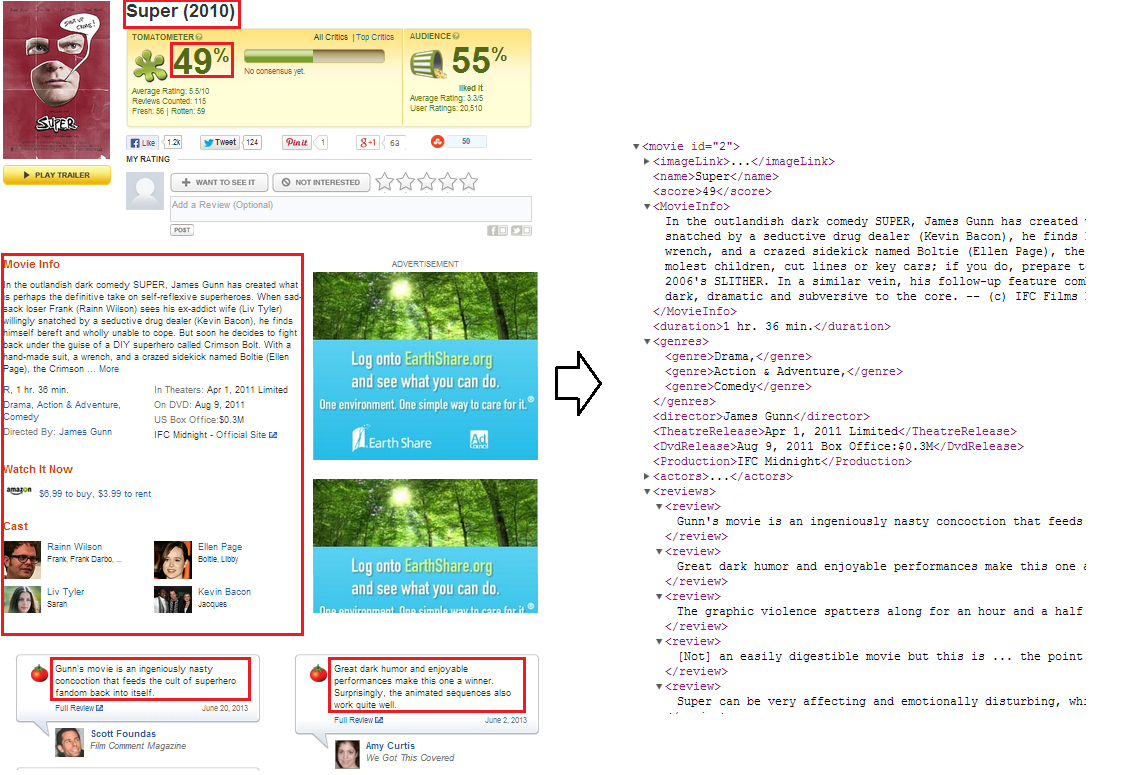
\includegraphics[width=4.5in]{rot.png}
    \caption{Collecting data from Rotten Tomatoes}
    \label{fig:xmlFile}
\end{figure}

\subsubsection{Evaluation \& Summary}
After several iterations, we collected 6227 movies each containing movie metadata and the reviews. We collected only top critics reviews because we feel that those are the most representative of all the reviews. As focused crawler parse all the content in documents and filter only the relevant content for the application, crawling took more time than a normal crawler would take. But the flexibility in the design of the crawler allowed us to run it in iterations so we did not face any issue regarding the time for crawling. We took 20 random samples from the file and compared the contents with the content in the site. In all the cases, we were able to capture all the relevant data needed for the search and sentiment analysis functionality.

\subsection{Lucene Search, Wildcard Queries \& Autocomplete : S.R. Patra}
\subsubsection{Motivation}
Lucene provides very rich library functions to implement indexing and search. So we implemented lucene search as a metric to evaluate our boolean and vector space model performances. 
\subsubsection{Approach}
Lucene.net library was used for generating the index and for getting the search results from the processed query. We limited our search results to be 10 top relevant results. Index was created for different fields to allow the user to search based on any criteria they want i.e. based on actor, director, genres etc. We also implemented the \textit{Autocomplete} feature to help the user with the query. This feature was developed in \textit{JQuery} and was implemented as a web service which queries the database about possible movie names after each input letter in the text box. 

\paragraph{}
Wild card queries were used to provide query suggestions to the user when the user only knows parts of the terms in the query. The speech to text query assistance feature was also included using the HTML5 Webkit speech. All the features discussed above are shown in fig.\ref{fig:search}.
\begin{figure}[H]
    \centering
    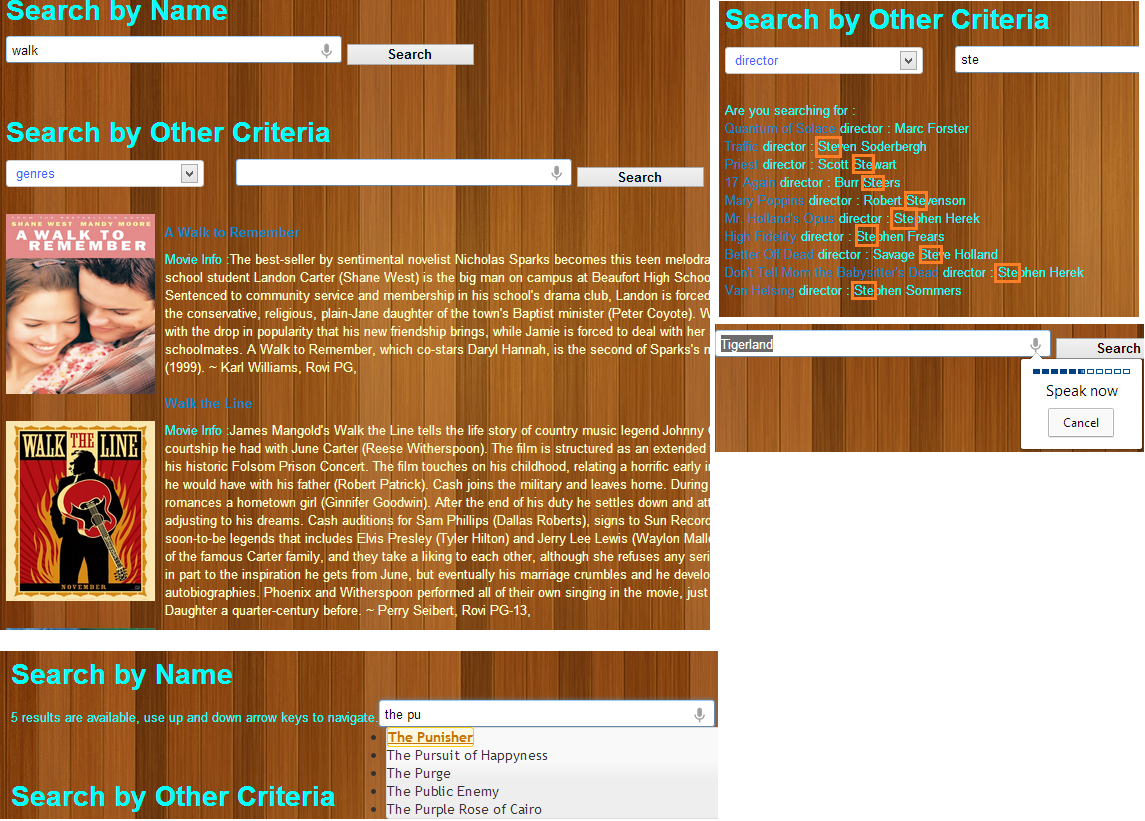
\includegraphics[width=4.5in]{search.png}
    \caption{Searching functionalities}
    \label{fig:search}
\end{figure}

\subsubsection{Evaluation \& Summary}
After trying a number of sample queries for different search criterias, we feel that the search provided quite relevant results in all the cases. The wildcard queries were also accurate in their suggestions and the users were able to retrieve relevant movie names based on parts of the search query terms. 
\subsection{Paragraph Level Sentiment Analysis : S.R. Patra}
\subsubsection{Motivation}
Performing sentiment analysis on movie reviews have  lot of advantages. Most of the users take opinion from others before going for a movie. If they want to research about a movie online, they have to spend time in reading the reviews or watching reviews in videos. In this context, a sentiment analyzer can help in saving time as it gives the users a score which represents the overall opinion of others about the movie. We also wanted to perform sentiment analysis on YouTube videos of different movie reviews because a large number of people also prefer to watch video reviews. 

\subsubsection{Approach}

We perform sentiment analysis task based on a naive Bayes classifier. It was implemented using a web service \textit{uClassify}\cite{uclassify} where the classifier \textit{ReviewClassifier} was trained with a dataset containing 1000 positive and 1000 negative review text files\cite{Dataset}. After the training, the classifier had 703414 negative features (words) whereof 37640 were unique and 798382 positive features whereof 40173 were unique. For each of these words, the classifier calculates polarity values which is basically a combination of a \textit{positive} and a \textit{negative} score.  The probability of a document being in a class, which is basically the product of the probabilities of all the terms in the document being in that class, is calculated using the \textit{Bayes theorem}. It can be better understood using the following example. Let us assume that a test document \textit{D} has 3 terms \textit{d1, d2 and d3}. The classifier calculates the probabilities of the document being in both the classes \textit{Positive} and \textit{Negative} and classifies them to be of the class having the higher probability score.

$$ P(D|Positive) = P(d1|Positive) * P(d2|Positive)* P(d3|Positive)$$
$$P(D|Negative) = P(d1|Negative) * P(d2|Negative)* P(d3|Negative)$$
\linebreak
If $P(D|Positive) > P(D|Negative)$, then the document is classified as \textit{Positive} else it is considered \textit{Negative}. 

\begin{figure}[H]
    \centering
    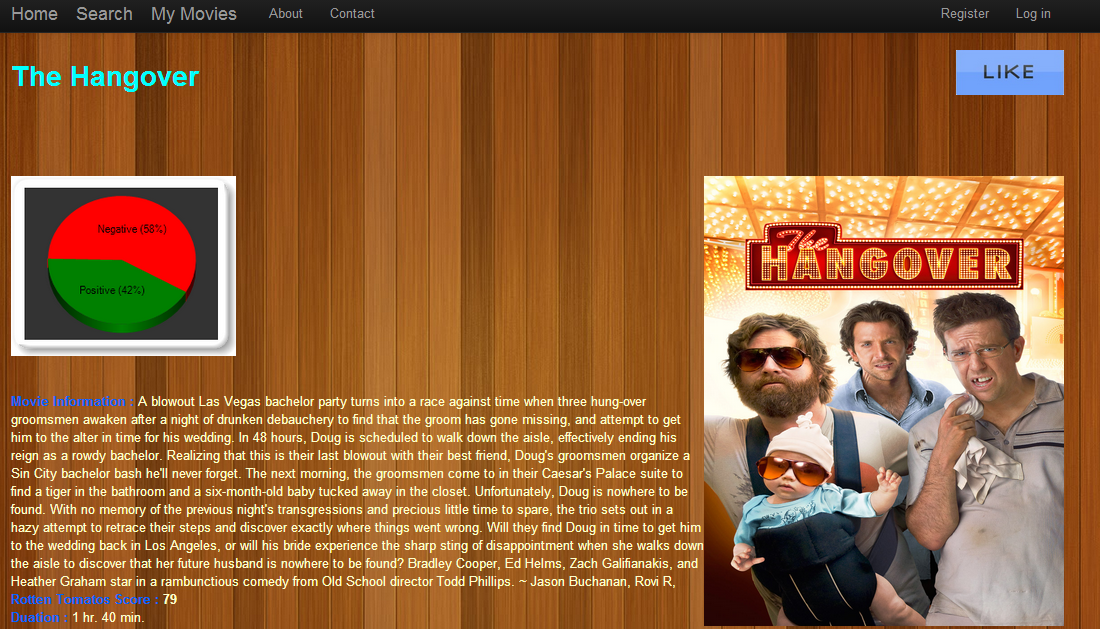
\includegraphics[width=4.0in]{score.png}
    \caption{Positive and Negative scores of the movie}
    \label{fig:score}
\end{figure}
We performed sentiment analysis on all the 6227 movies and probability scores are displayed in the page for each movie as shown in fig.\ref{fig:score}. To make our project more interactive, we also provide a functionality where the user can write a review of his own and get the polarity scores for the review. Additionally he has the option to \textit{submit} the review to the database as shown in fig.\ref{fig:review}.

\begin{figure}[H]
    \centering
    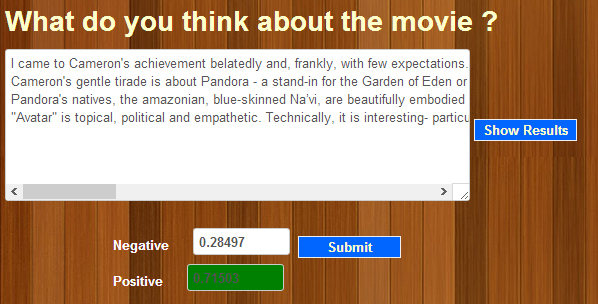
\includegraphics[width=4.0in]{review.png}
    \caption{User Review with option to submit}
    \label{fig:review}
    \end{figure}

We did not find any good dataset containing video reviews,so in our application, we decided to use YouTube API\cite{youtube2} to display top 6 video reviews of the movie. To analyze the content of these videos, we take the help of YouTube Closed Caption feature. Integrating \textit{Google2SRT} \cite{youtube} helped us get the closed captions of the video and perform sentiment analysis on them. Fig\ref{fig:youtube} displays a sample showing how the captions from the video are converted to text and how the scores are displayed post analysis.


\begin{figure}[H]
    \centering
    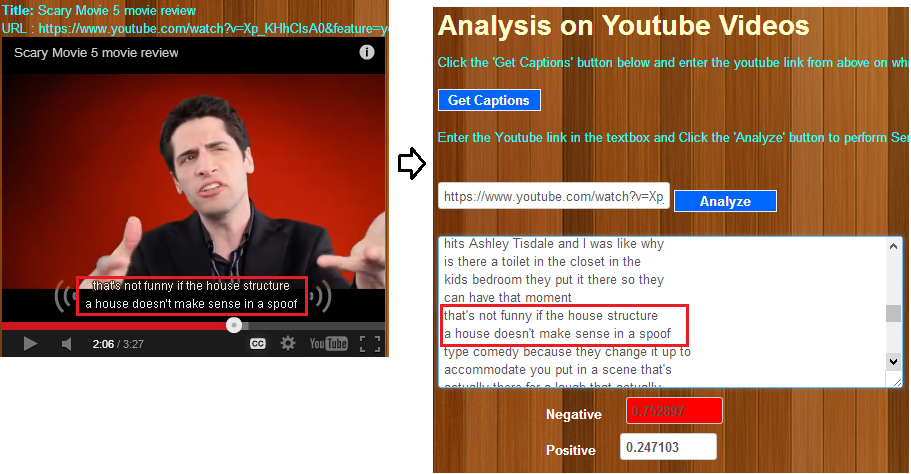
\includegraphics[width=4.0in]{youtube.png}
    \caption{Sentiment analysis on youtube videos}
    \label{fig:youtube}
    \end{figure}

\subsubsection{Challenges}
Performing sentiment analysis on YouTube videos itself is a really challenging task. because Closed caption is a new feature in YouTube and most of the older review videos are simply transcribed based on Speech to Text recognition technologies which are not always so accurate. Also, in videos, people generally tend to compare the movie with other movies which really affects the score. For example, if a user did not like previous X-Men movies but liked the new one and for more than half part of the video, he criticizes the previous parts, the video will be classified negative which should not be the case.

\subsubsection{Evaluation \& Summary}
For evaluation, we chose a metric where movies with positive score greater than 65\% were considered \textit{Positive} and less than 65\% were considered \textit{Negative}. From the Rotten Tomatoes website, we collected the percentage of positive reviews in the attribute \textit{score } and used the same metric for these scores. We were able to achieve 77.69\% Accuracy. Details are shown in fig.\ref{fig:confusion}. Considering the fact that we only collected the representative set of top critics reviews and not the complete set of reviews, we believe the results are quite satisfactory. Evaluation on YouTube videos were performed manually. We watched 10 random reviews and classified those videos. After comparing them with the scores from the classifier, 7 of them were correctly classified whereas 3 were classified in the wrong class.  
 
\begin{figure}[H]
    \centering
    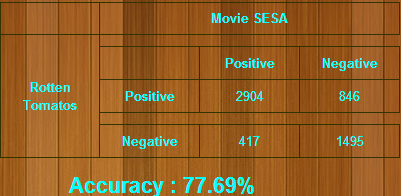
\includegraphics[width=4.0in]{confusion.png}
    \caption{Confusion Matrix of the classifier}
    \label{fig:confusion}
    \end{figure} 
    
 We also thought it would be interesting to analyze how popular are movies from different \textit{genres }. Figure \ref{fig:genres} 
 shows the results of our analysis.It can be seen that Drama movies are really popular with the highest number of positive reviews. 
 \begin{figure}[H]
    \centering
    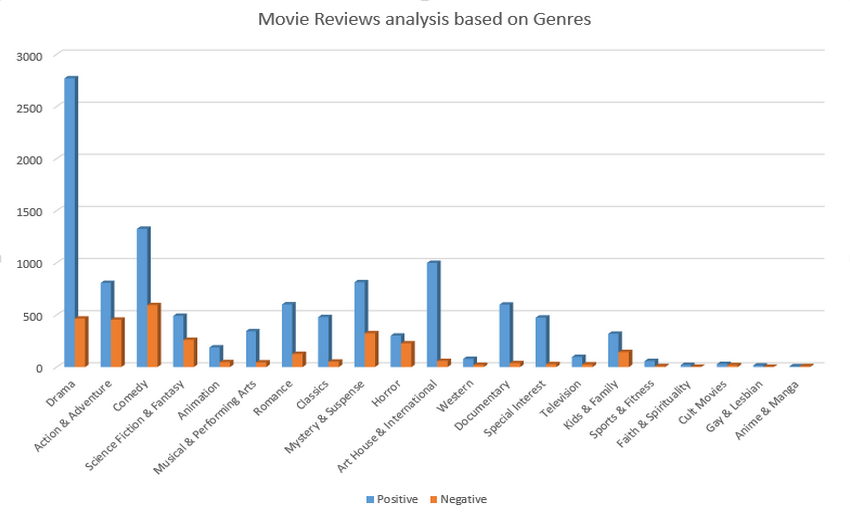
\includegraphics[width=3.5in]{genres.png}
    \caption{Movie reviews analysis based on genres}
    \label{fig:genres}
    \end{figure} 
    Figure \ref{fig:genres2} shows the percentage of positive and negative reviews per genre.
    \begin{figure}[H]
    \centering
    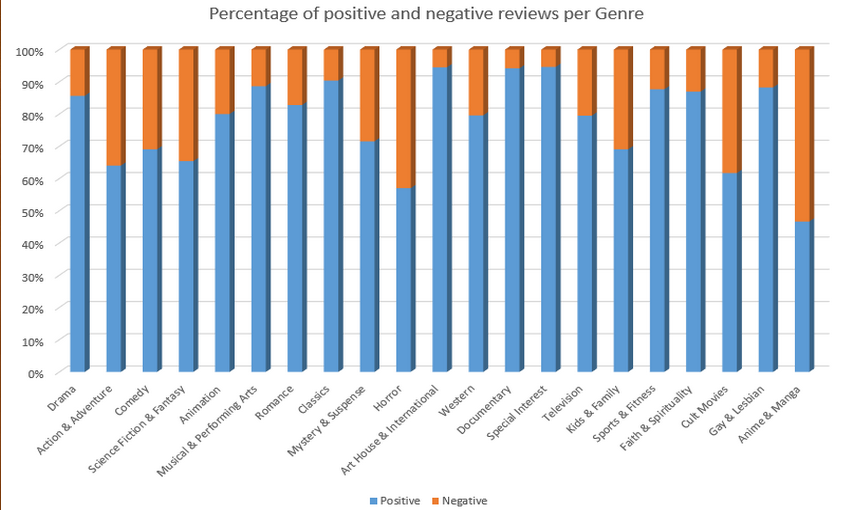
\includegraphics[width=3.5in]{genres2.png}
    \caption{Percentage of Positive and Negative reviews per genre}
    \label{fig:genres2}
    \end{figure} 
    
 \subsection{User Modeling \& Personalized Recommendations : S.R. Patra}    
 \subsubsection{Motivation}
 User modeling has become an integral part of web information systems these days. Personalized recommendations has  great impact in attracting new users to the site, because personalized approach has the best chance of predicting user's likes and dislikes and provide relevant recommendations. This motivated us to add a personalized recommendation component in our project.
 
  \subsubsection{Approach}
  Our approach is to obtain explicit feedback from the user about his fondness of the movies. We do this by providing a \textit{Like} button on each movie's page and by clicking this button , the user lets us know that (s)he likes the movie. For each user we store this information in a database table \textit{UserLikeMovies} and the user can always see the list of movies that he has liked in a separate page called \textit{My Movies}. Figure\ref{fig:like} shows how the component was integrated in our project. As can be seen from the figure, we use pie chart representation\cite{pie} to display the percentage distribution of the movies user liked from different genres. The genre that the user is most inclined towards is considered to be his category. We recommend the best 20 movies (based on the sentiment analysis scores) in that genre to the user. If the user is inclined towards 2 genres, he will get recommendations for both the genres. Also,gradually, if the user likes other kind of movies, his category will change and he will get recommendations from the new category.
  
  \begin{figure}[H]
    \centering
    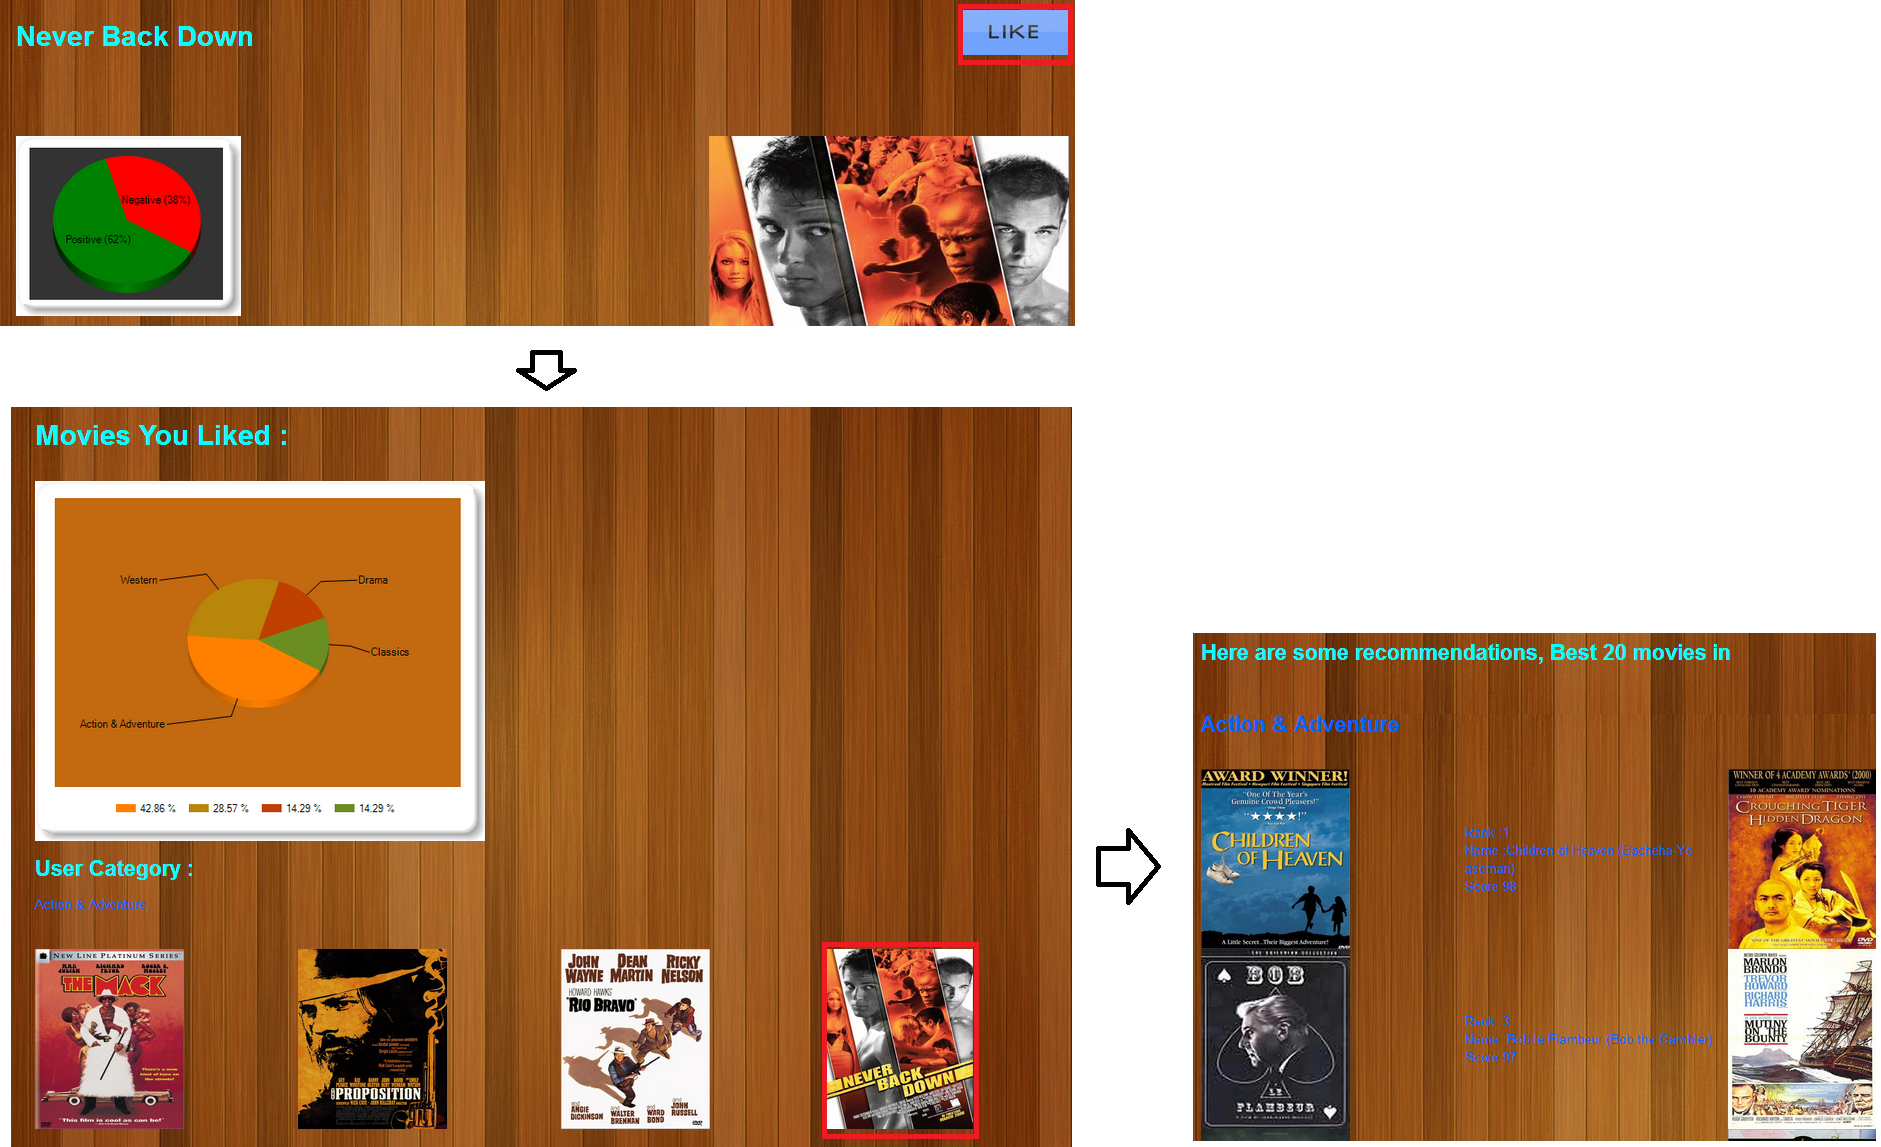
\includegraphics[width=5in]{like.png}
    \caption{Personalized recommendations}
    \label{fig:like}
    \end{figure} 
    
 \subsubsection{Summary}
 Our method could easily be modified to accommodate \textit{Fixed Training Window} approach to handle concept drift. Instead of performing the analysis on all the movies the user has liked, if we perform analysis on only last few movies (s)he liked, we can detect a concept drift and change user's category immediately to recommend movies based on new category.
\begin{thebibliography}{1}
\bibitem{uclassify} http://www.uclassify.com/
  \bibitem{Dataset} http://www.cs.cornell.edu/people/pabo/movie-review-data/
  
\bibitem{youtube} http://www.techreviewsdaily.com/how-to/google2srt-download-subtitles-from-youtube-videos-to-subrip-srt/

  \end{thebibliography}

\end{document}